\documentclass[a4paper,12pt]{article}
\usepackage{fullpage}
\usepackage{graphicx}
\usepackage{caption}
\usepackage{float}
\usepackage{hyperref}
\usepackage{tabularx}

\hypersetup{
    colorlinks,
    citecolor=blue,
    filecolor=black,
    linkcolor=blue,
    urlcolor=blue
}
\begin{document}
%\selectlanguage{english}
\pagenumbering{Roman}



\title{\begin{Huge}
\textbf{Use Case: Simulation Platform for Smart Fridge and Sudoku Solver}
\end{Huge}}
\author{\begin{Large}
Sreenivas, Jonas and Mariusz
\end{Large}}
\date{\today}
\maketitle
\thispagestyle{empty}

\newpage

\pagenumbering{arabic}
\section{Purpose}
This document provides use cases for the simulation platform for rottening fruits and Sudokus. The use cases are described either by words and a UML diagram.

\section{Use Case}
\subsection{Specifications}

\begin{tabularx}{\linewidth}{|l|l|X|}
\hline
\textbf{Number} & \multicolumn{2}{l|}{1} \\
\hline
\textbf{Name} & \multicolumn{2}{l|}{Rendering images for SmartFridge} \\
\hline
\textbf{Description} &  \multicolumn{2}{X|}{A User goes through the dialogues to create an image containing various fruits of different rotten and non-rotten states.} \\
\hline
\textbf{Priority} & \multicolumn{2}{l|}{5} \\
\hline
\textbf{Preconditions} & \multicolumn{2}{l|}{Program was started} \\
\hline
\textbf{Postconditions} & \multicolumn{2}{l|}{None} \\
\hline
\textbf{Primary Actor(s)} & \multicolumn{2}{l|}{User} \\
\hline
\textbf{Secondary Actor(s)} & \multicolumn{2}{l|}{None} \\
\hline
\textbf{Trigger} & \multicolumn{2}{l|}{User chooses SmartFridge after program start.} \\
\hline
\textbf{Main Scenario} & Step & Action\\
\hline
 & 1 & Program shows start dialogue containing buttons for choice between SmartFridge and Sudoku\\
\cline{2-3}
 & 2 & User chooses SmartFridge\\
\cline{2-3}
 & 3 & Program displays parameter selection with default values\\
\cline{2-3}
 & 4 & User changes parameters at will \\
\cline{2-3}
 & 5 & Program displays rendered image for given input parameters \\
\cline{2-3}
 & 6 & User chooses whether to reject or save the image \\
\hline
\textbf{Extensions} & \textbf{Step} & \textbf{Branching Action} \\
\hline
& 4.1 & User insert number and sort of fruit. \\
\cline{2-3}
& 4.2 & Program shows preview of the scene to render \\
\hline
\textbf{Issues} & \multicolumn{2}{X|}{How does the selection look like? Does the user click through multiple images or does he get only one image per generation?} \\
\hline
\end{tabularx}
 \\
 \\
 \\
\begin{tabularx}{\linewidth}{|l|l|X|}
\hline
\textbf{Number} & \multicolumn{2}{l|}{2} \\
\hline
\textbf{Name} & \multicolumn{2}{l|}{Rendering images for Sudoku Solver} \\
\hline
\textbf{Description} &  \multicolumn{2}{X|}{A User goes through the dialogues to create an image dataset containing various Sudoku puzzles.} \\
\hline
\textbf{Priority} & \multicolumn{2}{l|}{4} \\
\hline
\textbf{Preconditions} & \multicolumn{2}{l|}{Program was started} \\
\hline
\textbf{Postconditions} & \multicolumn{2}{l|}{None} \\
\hline
\textbf{Primary Actor(s)} & \multicolumn{2}{l|}{User} \\
\hline
\textbf{Secondary Actor(s)} & \multicolumn{2}{l|}{None} \\
\hline
\textbf{Trigger} & \multicolumn{2}{l|}{User chooses Sudoku after program start.} \\
\hline
\textbf{Main Scenario} & \textbf{Step} & \textbf{Action} \\
\hline
 & 1 & Program shows start dialogue containing buttons for choice between SmartFridge and Sudoku\\
\cline{2-3}
 & 2 & User chooses Sudoku \\
\cline{2-3}
 & 3 & Program displays parameter selection with default values\\
\cline{2-3}
 & 4 & User changes parameters at will \\
\cline{2-3}
 & 5 & Program displays rendered image for given input parameters \\
\cline{2-3}
 & 6 & User chooses whether to reject or save image \\
\hline
\textbf{Extensions} & \textbf{Step} & \textbf{Branching Action} \\
\hline
& 4.1 & Program shows preview of the Sudoku scene to render. \\
\hline
\textbf{Issues} & \multicolumn{2}{X|}{How does the selection look like? Does the user click through multiple images or does he get only one image per generation?} \\
\hline
\end{tabularx}
 \\
 \\
 \\
\begin{tabularx}{\linewidth}{|l|l|X|}
\hline
\textbf{Number} & \multicolumn{2}{l|}{3} \\
\hline
\textbf{Name} & \multicolumn{2}{X|}{Add a fruit to the SmartFridge (Experimental Use case for scalability in future} \\
\hline
\textbf{Description} &  \multicolumn{2}{X|}{A Developer goes through the dialogues to create an image containing one Sudoku.} \\
\hline
\textbf{Priority} & \multicolumn{2}{l|}{2} \\
\hline
\textbf{Preconditions} & \multicolumn{2}{l|}{Developer has information and access to plugin interface} \\
\hline
\textbf{Postconditions} & \multicolumn{2}{l|}{Program is still executable} \\
\hline
\textbf{Primary Actor(s)} & \multicolumn{2}{l|}{Developer} \\
\hline
\textbf{Secondary Actor(s)} & \multicolumn{2}{l|}{None} \\
\hline
\textbf{Trigger} & \multicolumn{2}{l|}{None} \\
\hline
\textbf{Main Scenario} & \textbf{Step} & \textbf{Action} \\
\hline
 & 1 & Developer adds a blender compatible mesh for the new fruit\\
\cline{2-3}
 & 2 & Developer adds a colormap for the new fruit \\
\hline
\textbf{Extensions} & \textbf{Step} & \textbf{Branching Action} \\
\hline
& 1.1 & The developer has to apply the parameter types and names for his mesh generating routine \\
\hline
\textbf{Issues} & \multicolumn{2}{X|}{How does the selection look like? Does the user click through multiple images or does he get only one image per generation?} \\
\hline
\end{tabularx}
\subsection{UML diagram}
\begin{figure}[H]
\centering
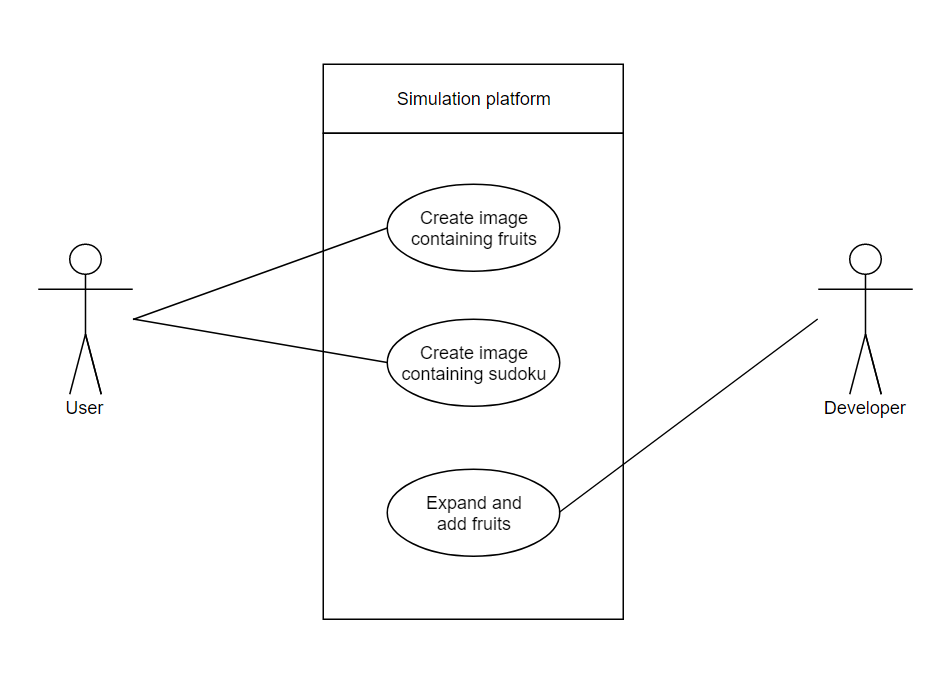
\includegraphics[scale=0.65]{usecase_new_1.png}
\caption{Use Case UML diagram}
\end{figure}
\end{document}
